% Options for packages loaded elsewhere
\PassOptionsToPackage{unicode}{hyperref}
\PassOptionsToPackage{hyphens}{url}
\PassOptionsToPackage{dvipsnames,svgnames,x11names}{xcolor}
%
\documentclass[
  letterpaper,
  DIV=11]{scrreprt}

\usepackage{amsmath,amssymb}
\usepackage{iftex}
\ifPDFTeX
  \usepackage[T1]{fontenc}
  \usepackage[utf8]{inputenc}
  \usepackage{textcomp} % provide euro and other symbols
\else % if luatex or xetex
  \usepackage{unicode-math}
  \defaultfontfeatures{Scale=MatchLowercase}
  \defaultfontfeatures[\rmfamily]{Ligatures=TeX,Scale=1}
\fi
\usepackage{lmodern}
\ifPDFTeX\else  
    % xetex/luatex font selection
\fi
% Use upquote if available, for straight quotes in verbatim environments
\IfFileExists{upquote.sty}{\usepackage{upquote}}{}
\IfFileExists{microtype.sty}{% use microtype if available
  \usepackage[]{microtype}
  \UseMicrotypeSet[protrusion]{basicmath} % disable protrusion for tt fonts
}{}
\makeatletter
\@ifundefined{KOMAClassName}{% if non-KOMA class
  \IfFileExists{parskip.sty}{%
    \usepackage{parskip}
  }{% else
    \setlength{\parindent}{0pt}
    \setlength{\parskip}{6pt plus 2pt minus 1pt}}
}{% if KOMA class
  \KOMAoptions{parskip=half}}
\makeatother
\usepackage{xcolor}
\setlength{\emergencystretch}{3em} % prevent overfull lines
\setcounter{secnumdepth}{5}
% Make \paragraph and \subparagraph free-standing
\ifx\paragraph\undefined\else
  \let\oldparagraph\paragraph
  \renewcommand{\paragraph}[1]{\oldparagraph{#1}\mbox{}}
\fi
\ifx\subparagraph\undefined\else
  \let\oldsubparagraph\subparagraph
  \renewcommand{\subparagraph}[1]{\oldsubparagraph{#1}\mbox{}}
\fi

\usepackage{color}
\usepackage{fancyvrb}
\newcommand{\VerbBar}{|}
\newcommand{\VERB}{\Verb[commandchars=\\\{\}]}
\DefineVerbatimEnvironment{Highlighting}{Verbatim}{commandchars=\\\{\}}
% Add ',fontsize=\small' for more characters per line
\usepackage{framed}
\definecolor{shadecolor}{RGB}{241,243,245}
\newenvironment{Shaded}{\begin{snugshade}}{\end{snugshade}}
\newcommand{\AlertTok}[1]{\textcolor[rgb]{0.68,0.00,0.00}{#1}}
\newcommand{\AnnotationTok}[1]{\textcolor[rgb]{0.37,0.37,0.37}{#1}}
\newcommand{\AttributeTok}[1]{\textcolor[rgb]{0.40,0.45,0.13}{#1}}
\newcommand{\BaseNTok}[1]{\textcolor[rgb]{0.68,0.00,0.00}{#1}}
\newcommand{\BuiltInTok}[1]{\textcolor[rgb]{0.00,0.23,0.31}{#1}}
\newcommand{\CharTok}[1]{\textcolor[rgb]{0.13,0.47,0.30}{#1}}
\newcommand{\CommentTok}[1]{\textcolor[rgb]{0.37,0.37,0.37}{#1}}
\newcommand{\CommentVarTok}[1]{\textcolor[rgb]{0.37,0.37,0.37}{\textit{#1}}}
\newcommand{\ConstantTok}[1]{\textcolor[rgb]{0.56,0.35,0.01}{#1}}
\newcommand{\ControlFlowTok}[1]{\textcolor[rgb]{0.00,0.23,0.31}{#1}}
\newcommand{\DataTypeTok}[1]{\textcolor[rgb]{0.68,0.00,0.00}{#1}}
\newcommand{\DecValTok}[1]{\textcolor[rgb]{0.68,0.00,0.00}{#1}}
\newcommand{\DocumentationTok}[1]{\textcolor[rgb]{0.37,0.37,0.37}{\textit{#1}}}
\newcommand{\ErrorTok}[1]{\textcolor[rgb]{0.68,0.00,0.00}{#1}}
\newcommand{\ExtensionTok}[1]{\textcolor[rgb]{0.00,0.23,0.31}{#1}}
\newcommand{\FloatTok}[1]{\textcolor[rgb]{0.68,0.00,0.00}{#1}}
\newcommand{\FunctionTok}[1]{\textcolor[rgb]{0.28,0.35,0.67}{#1}}
\newcommand{\ImportTok}[1]{\textcolor[rgb]{0.00,0.46,0.62}{#1}}
\newcommand{\InformationTok}[1]{\textcolor[rgb]{0.37,0.37,0.37}{#1}}
\newcommand{\KeywordTok}[1]{\textcolor[rgb]{0.00,0.23,0.31}{#1}}
\newcommand{\NormalTok}[1]{\textcolor[rgb]{0.00,0.23,0.31}{#1}}
\newcommand{\OperatorTok}[1]{\textcolor[rgb]{0.37,0.37,0.37}{#1}}
\newcommand{\OtherTok}[1]{\textcolor[rgb]{0.00,0.23,0.31}{#1}}
\newcommand{\PreprocessorTok}[1]{\textcolor[rgb]{0.68,0.00,0.00}{#1}}
\newcommand{\RegionMarkerTok}[1]{\textcolor[rgb]{0.00,0.23,0.31}{#1}}
\newcommand{\SpecialCharTok}[1]{\textcolor[rgb]{0.37,0.37,0.37}{#1}}
\newcommand{\SpecialStringTok}[1]{\textcolor[rgb]{0.13,0.47,0.30}{#1}}
\newcommand{\StringTok}[1]{\textcolor[rgb]{0.13,0.47,0.30}{#1}}
\newcommand{\VariableTok}[1]{\textcolor[rgb]{0.07,0.07,0.07}{#1}}
\newcommand{\VerbatimStringTok}[1]{\textcolor[rgb]{0.13,0.47,0.30}{#1}}
\newcommand{\WarningTok}[1]{\textcolor[rgb]{0.37,0.37,0.37}{\textit{#1}}}

\providecommand{\tightlist}{%
  \setlength{\itemsep}{0pt}\setlength{\parskip}{0pt}}\usepackage{longtable,booktabs,array}
\usepackage{calc} % for calculating minipage widths
% Correct order of tables after \paragraph or \subparagraph
\usepackage{etoolbox}
\makeatletter
\patchcmd\longtable{\par}{\if@noskipsec\mbox{}\fi\par}{}{}
\makeatother
% Allow footnotes in longtable head/foot
\IfFileExists{footnotehyper.sty}{\usepackage{footnotehyper}}{\usepackage{footnote}}
\makesavenoteenv{longtable}
\usepackage{graphicx}
\makeatletter
\def\maxwidth{\ifdim\Gin@nat@width>\linewidth\linewidth\else\Gin@nat@width\fi}
\def\maxheight{\ifdim\Gin@nat@height>\textheight\textheight\else\Gin@nat@height\fi}
\makeatother
% Scale images if necessary, so that they will not overflow the page
% margins by default, and it is still possible to overwrite the defaults
% using explicit options in \includegraphics[width, height, ...]{}
\setkeys{Gin}{width=\maxwidth,height=\maxheight,keepaspectratio}
% Set default figure placement to htbp
\makeatletter
\def\fps@figure{htbp}
\makeatother
% definitions for citeproc citations
\NewDocumentCommand\citeproctext{}{}
\NewDocumentCommand\citeproc{mm}{%
  \begingroup\def\citeproctext{#2}\cite{#1}\endgroup}
\makeatletter
 % allow citations to break across lines
 \let\@cite@ofmt\@firstofone
 % avoid brackets around text for \cite:
 \def\@biblabel#1{}
 \def\@cite#1#2{{#1\if@tempswa , #2\fi}}
\makeatother
\newlength{\cslhangindent}
\setlength{\cslhangindent}{1.5em}
\newlength{\csllabelwidth}
\setlength{\csllabelwidth}{3em}
\newenvironment{CSLReferences}[2] % #1 hanging-indent, #2 entry-spacing
 {\begin{list}{}{%
  \setlength{\itemindent}{0pt}
  \setlength{\leftmargin}{0pt}
  \setlength{\parsep}{0pt}
  % turn on hanging indent if param 1 is 1
  \ifodd #1
   \setlength{\leftmargin}{\cslhangindent}
   \setlength{\itemindent}{-1\cslhangindent}
  \fi
  % set entry spacing
  \setlength{\itemsep}{#2\baselineskip}}}
 {\end{list}}
\usepackage{calc}
\newcommand{\CSLBlock}[1]{\hfill\break\parbox[t]{\linewidth}{\strut\ignorespaces#1\strut}}
\newcommand{\CSLLeftMargin}[1]{\parbox[t]{\csllabelwidth}{\strut#1\strut}}
\newcommand{\CSLRightInline}[1]{\parbox[t]{\linewidth - \csllabelwidth}{\strut#1\strut}}
\newcommand{\CSLIndent}[1]{\hspace{\cslhangindent}#1}

\KOMAoption{captions}{tableheading}
\makeatletter
\@ifpackageloaded{bookmark}{}{\usepackage{bookmark}}
\makeatother
\makeatletter
\@ifpackageloaded{caption}{}{\usepackage{caption}}
\AtBeginDocument{%
\ifdefined\contentsname
  \renewcommand*\contentsname{Inhaltsverzeichnis}
\else
  \newcommand\contentsname{Inhaltsverzeichnis}
\fi
\ifdefined\listfigurename
  \renewcommand*\listfigurename{Abbildungsverzeichnis}
\else
  \newcommand\listfigurename{Abbildungsverzeichnis}
\fi
\ifdefined\listtablename
  \renewcommand*\listtablename{Tabellenverzeichnis}
\else
  \newcommand\listtablename{Tabellenverzeichnis}
\fi
\ifdefined\figurename
  \renewcommand*\figurename{Abbildung}
\else
  \newcommand\figurename{Abbildung}
\fi
\ifdefined\tablename
  \renewcommand*\tablename{Tabelle}
\else
  \newcommand\tablename{Tabelle}
\fi
}
\@ifpackageloaded{float}{}{\usepackage{float}}
\floatstyle{ruled}
\@ifundefined{c@chapter}{\newfloat{codelisting}{h}{lop}}{\newfloat{codelisting}{h}{lop}[chapter]}
\floatname{codelisting}{Listing}
\newcommand*\listoflistings{\listof{codelisting}{Listingverzeichnis}}
\makeatother
\makeatletter
\makeatother
\makeatletter
\@ifpackageloaded{caption}{}{\usepackage{caption}}
\@ifpackageloaded{subcaption}{}{\usepackage{subcaption}}
\makeatother
\ifLuaTeX
\usepackage[bidi=basic]{babel}
\else
\usepackage[bidi=default]{babel}
\fi
\babelprovide[main,import]{ngerman}
% get rid of language-specific shorthands (see #6817):
\let\LanguageShortHands\languageshorthands
\def\languageshorthands#1{}
\ifLuaTeX
  \usepackage{selnolig}  % disable illegal ligatures
\fi
\usepackage{bookmark}

\IfFileExists{xurl.sty}{\usepackage{xurl}}{} % add URL line breaks if available
\urlstyle{same} % disable monospaced font for URLs
\hypersetup{
  pdftitle={MTRS-Skript},
  pdfauthor={Leopold Götsch},
  pdflang={de},
  colorlinks=true,
  linkcolor={blue},
  filecolor={Maroon},
  citecolor={Blue},
  urlcolor={Blue},
  pdfcreator={LaTeX via pandoc}}

\title{MTRS-Skript}
\author{Leopold Götsch}
\date{2024-03-08}

\begin{document}
\maketitle

\renewcommand*\contentsname{Inhaltsverzeichnis}
{
\hypersetup{linkcolor=}
\setcounter{tocdepth}{2}
\tableofcontents
}
\bookmarksetup{startatroot}

\chapter*{Willkommen zum Skript}\label{willkommen-zum-skript}
\addcontentsline{toc}{chapter}{Willkommen zum Skript}

\markboth{Willkommen zum Skript}{Willkommen zum Skript}

Dieses Skriptum dient zu Unterstützung und Ergänzung der Inhalte aus dem
Unterricht. Der ``rote Faden'' im Unterricht ist in den jeweiligen
Klassennotizbüchern zu finden. Darin sind auch Links zu den passenden
Kapiteln in diesem Skript zu finden. Das Skriptum wird ständig erweitert
und verbessert. Input ist willkommen.

\section*{Verbessern}\label{verbessern}
\addcontentsline{toc}{section}{Verbessern}

\markright{Verbessern}

Ich freue mich über alle Fehlerkorrekturen und Verbesserungsvorschläge
die mich erreichen. Am einfachsten ist dies via Mail.

\section*{Mitwirken}\label{mitwirken}
\addcontentsline{toc}{section}{Mitwirken}

\markright{Mitwirken}

Wer am Skriptum mitarbeiten möchte kann mich gerne kontaktieren. Meine
Kontaktdaten sind auf der Homepage der HTL-Anichstrasse zu finden.

Viel Vergnügen mit MTRS und dem interaktiven Quarto Book!

\part{Steuer- und Regelungstechnik}

In diesem Kapitel geht es darum wie wir Maschinen und Schaltungen dazu
bringen, ein gewünschtes Verhalten zu zeigen. Zum Beipiel soll ein
Roboterarm ein Werkstück von der Position A zur Position B stellen. Oder
eine Drohne trotz Windes ihre Postion halten.\\
Wir sprechen von \textbf{Steuern}, wenn wir eine Befehlskette vorgeben
und keine Möglichkeit haben auf Störungen einfluss zu nehmen.\\
Von \textbf{Regeln} sprechen wir, wenn wir Informationen über das zu
erreichende Ziel erhalten und damit auf Störungen eingehen können. Es
gibt beim Regeln daher eine Feedbackschleife oder auch Rückkopplung
genannt.

\chapter{Regelungstechnik}\label{regelungstechnik}

In diesem Teil des Skriptums geht es darum wie wir Maschinen und
Schaltungen dazu bringen, trotz Störeinflüssen das gewünsche Verhalten
zu Zeigen. Zum Beipiel soll ein Tempomant des Autos die Geschwindigkeit
halten, trotz starkem Gegenwindes. Es werden die Grundlagen der
Regelungstechnik vermittelt. Dabei wird das theoretische Wissen anhand
konkreter Anwendungen erarbeitet.

\section{Warum wir regeln}\label{warum-wir-regeln}

Viele Aufgaben von Maschinen können auch durch Steuern umgesetzt werden.
Eine Regelung erlaubt es aber, auf unerwünschte Einflüsse, sogenannte
Störgrößen, zu reagieren. Als Beispiel soll der Tempomat,
Geschwindigkeitsregelanlage, des Autos dienen. Die Aufgabe des
Tempomates ist es, die Geschwindigkeit, Regelgröße, konstant zu halten.
Als unerwünschte Einflüsse, Störgrößen, sind alle physikalischen Größen
zu betrachten, welche die Geschwindigkeit beeinflussen. Beispiele sind
die Steigung der Straße und Wind.\\
Die Geschwindigkeit des Autos wird über die Leistung, Stellgröße,
bestimmt. Führt die Straße Bergauf wird mehr Leistung für die gleiche
Geschwindigkeit benötigt. Es muss also die Leistung laufend angepasst
werden, um eine konstante Geschwindigkeit zu erhalten.\\
Bei einer Steuerung würde eine Leistung eingestellt werden und sich
daraus eine Geschwindigkeit ergeben. Dieses wäre jedoch nur für einen
voreingestellten Fall identisch mit der gewünschten Geschwindigkeit.

\section{Wie wir regeln - Der
Standardregelkreis}\label{wie-wir-regeln---der-standardregelkreis}

Regeln ist ein Vorgang, bei dem der IST-Wert einer Größe gemessen und,
durch Nachstellen der Stellgröße, dem SOLL-Wert angeglichen wird.\\
Dazu wird das Ergebnis an den Eingang zurück geführt und vom Sollwert
subtrahiert. Es entsteht eine Rückkopplung. Durch das negative
Vorzeichen handelt es sich um eine Rückkopplung im Spezialfall einer
Gegenkopplung. Die Differenz aus dem Sollwert und dem zurückgeführten
Istwert ist die sogenannte Regelabweichung welche über den Regler zur
Stellgröße wird. Die Stellgröße ist nun die physikalische Größe die die
Regelstrecke zum gewünschten Verhalten führt.

\begin{figure}

\centering{

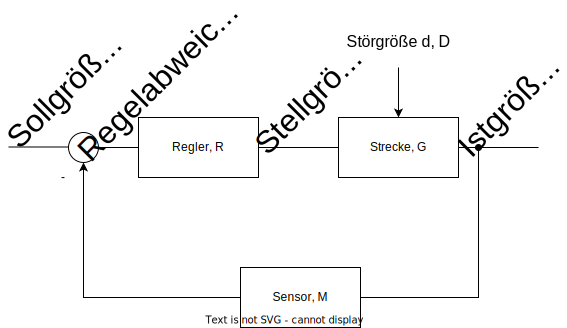
\includegraphics{SteuerRegel/images/Vollsändiger_Regelkreis.pdf}

}

\caption{\label{fig-Regelkreis}Standardregelkreis}

\end{figure}%

\subsection{Reglertypen}\label{reglertypen}

Es kann zwischen zwei Arten von Reglern unterschieden werden. Erstere
sind einfache Regler die die Stellgröße nur zwischen verschiedenen
Zuständen hin und her Schalten können. Zum Beispiel Ein / Aus. Oder die
Gänge eines Automatikgetriebes. Diese Regler werden \textbf{unstetige
Regler} genannt. Unstetige Regler können gut mittels Hysteresen
beschrieben werden.\\
Der zweite Typ von Regler kann die Stellgröße kontinurierlich anpassen.
Diese Regler werden \textbf{stetige Regler} genannt. Stetige Regler
können gut mit mathematische Gleichungen im Laplacebereich beschrieben
werden.

\section{Unstetige Regler}\label{unstetige-regler}

Klassische unstetige Regler sind Bimetallschalter. Diese werden zum
Beipiel bei Heizlüftern eingesetzt.\\
Ist der Raum, und damit das Bimetall kalt so ist der Kontakt geschlossen
und der Lüfter läuft. Wird die Raumluft und damit das Bimetall warm wird
der Kontakt geöffnet und der Lüfter hört auf zu heizen.

\(T_{ref}\) \ldots{} Referenz Temperatur

\(T\) \ldots{} Temperatur

\(T_{aus}\) \ldots{} Ausschaltschwelle

\(T_{ein}\) \ldots{} Einschaltschwelle

\begin{figure}

\centering{

\includegraphics{SteuerRegel/01.02_Regelungstechnik_files/figure-pdf/fig-zweipunktreglerplot-output-1.pdf}

}

\caption{\label{fig-zweipunktreglerplot}Zweipunktregler eines einfachen
Heizlüfters}

\end{figure}%

\subsection{Zweipunktregler}\label{zweipunktregler}

Der Zweipunktregler kann, wie der Name schon sagt, die Stellgröße
zwischen zwei Zuständen schalten. Zum Beipiel die Heizung einschalten
wenn die Temperatur zu niedrig ist und wieder Abschalten wenn die
Temperatur hoch genug ist. Siehe dazu die Kennlinie
Abbildung~\ref{fig-zweipunktreglerplot}. Die Kennlinie stellt eine
Hysterese dar. Die Umsetzung ist auch mittels Operationsverstärker
möglich.

\section{Stetige Regler}\label{stetige-regler}

Für das Verständnis von stetigen Reglern ist es hilfreich die
Regelungstechnik mathematisch zu betrachten, da sich ein Regler sehr gut
mit Formeln beschreiben und erklären lässt. In einem eigenen Kapitel
soll behandelt werden wie Regler praxisnahe implementiert werden
können.\\
Der oben gezeigte Regelkreis, Abbildung~\ref{fig-Regelkreis}, lässt sich
mathematisch als Übertragungsfunktion beschreiben. Hier werden
ausschließlich SISO (Single Input Single Output) und LTI (Linear Time
Invariant) Systeme betrachtet. Das Bedeutet Systeme die einen Eingang
und einen Ausgang haben. Jeder Block kann einzeln mit einer
Übertragungsfunktion, analog der Vierpoltheorie, beschrieben werden. Wie
auch in der Vierpoltheorie kann aber auch eine Verschaltung von Blöcken
als Übertragungsfunktion beschrieben werden. Ein Block wird in der
Regelungstechnik auch als \textbf{Strecke} bezeichnet.

\subsection{Die Übertragungsfunktion}\label{die-uxfcbertragungsfunktion}

\subsubsection{Motivation}\label{motivation}

Die Übertragungsfunktion Beschreibt den Zusammenhang zwischen Ausgang
und Eingang.\\
Ist die Übertragungsfunktion bekannt, so kann die Strecke und deren
Verhalten (der Ausgang) auf verschiedene Eingänge berechnet werden. Dies
wird auch Simulation genannt. Für Marketingzwecke könnte die
Übertragungsfunktion auch als einfache Form eines ``digitalen
Zwillings'' bezeichnet werden. Ist die Übertragungsfunktion mathematisch
beschrieben, können Regler entworfen und getestet werden, ohne das
tatsächliche physikalische Modell benutzen zu müssen. Dies ist speziell
sinnvoll wenn, das physikalische System für Testzwecke nicht zur
Verfügung steht bzw. nicht für Testzwecke geeignet ist. Eine Strecke
(=physikalisches System) steht z.B. nicht zur Verfügung, wenn:

\begin{itemize}
\tightlist
\item
  Es sich geographisch woanders befindet\\
\item
  Es für die Produktion benötigt wird\\
\item
  Es noch nicht gebaut wurde
\end{itemize}

Eine Strecke (=physikalisches System) ist nicht geeignet für Testzwecke
wenn z.B.:

\begin{itemize}
\tightlist
\item
  Das System sehr langsam ist (Heizung eines Gebäudes)\\
\item
  Ein fehlerhafter Regler großen Schaden anrichten kann
\end{itemize}

\subsubsection{Streckenidentifikation}\label{sec-Streckenidentifikation}

Als Streckenidentifiaktion wird der Vorgang beschrieben, von einem
physikalischem System das mathematische Modell, die
Übertragungsfunktion, zu erstellen. Zwei Methoden wie dieses Ziel
erreicht werden kann, werden hier beschrieben.

\begin{itemize}
\tightlist
\item
  Der mathematische Ansatz,
  Kapitel~\ref{sec-MathStreckenidentifikation}\\
\item
  Der messtechnische Ansatz,
  Kapitel~\ref{sec-MessStreckenidentifikation}
\end{itemize}

\begin{equation}\phantomsection\label{eq-EVA}{
V = \frac{A}{E}
}\end{equation}

\(E\) \ldots{} Eingang

\(A\) \ldots{} Ausgang

\(V\) \ldots{} Verarbeitung, die Übertragungsfunktion

Gängige Bezeichnungen der Übertragungsfunktion der einzelnen Blöcke ist
wie folgt.

\(G\) \ldots{} Übertragungsfunktion der zu Regelnden Strecke

\(R\) \ldots{} Übertragungsfunktion des Reglers

\(M\) \ldots{} Übertragungsfunktion des Sensors

\subsection{Mathematische
Streckenidentifikation}\label{sec-MathStreckenidentifikation}

Aus den physikalischen Zusammenhängen kann die Übertragungsfunktion
berechnet werden. Die komplexe Schreibweise ist nur für periodische
sinusförmige Signale geeignet. Sollen Signale betrachtet werden die
beliebig, stetig, sind ist die komplexe schreibweise nicht ausreichend.
Es müssen die physikalischen Gleichungen in differentieller Form
angeschrieben werden.

Um die Mathematik möglichst einfach zu halten wird in der
Regelungstechnik im Laplace Bereich gearbeitet. Dadurch ist es nicht
notwendig die Diffenrentialgleichung bei physikalischen Systemen, die
durch eine Differentialgleichung beschrieben werden, zu lösen.

Ein Besipiel, wie eine mathematische Streckenidentifikation abläuft ist
in Abschnitt Kapitel~\ref{sec-Laplace} zu finden.

\subsection{Messtechnische
Streckenidentifikation}\label{sec-MessStreckenidentifikation}

Manche Systeme sind zu komplex um Sie mathematisch zu beschreiben.
Andere Systeme sind mathematisch nicht beschreibbar, weil das Innenleben
nicht bekannt ist. In diesen Fällen kann die messtechnische Ermittlung
der Übertragungsfunktion herangezogen werden.\\
Dabei wird am Eingang der Strecke ein Testssignal aufgeschalten und der
Ausgang gemessen. Aus diesen Messdaten kann die Übertragungsfunktion,
ein mathemtisches Modell, der Strecke erstellt werden.

\subsection{Die Laplace Transformation}\label{sec-Laplace}

oder die Anstrengung der Faulen.

\subsubsection{Warum Laplace}\label{warum-laplace}

Um eine Übertragungsfunktion zu Berechnen muss der Ausgang durch den
Eingang dividiert werden. Wird das physikalische System durch eine
lineare Gleichung beschrieben ist das sehr Einfach möglich und die
Laplace Transformation ist nicht notwendig. Ein Beispiel dafür is das
Ohm'sche Gesetz.

\begin{equation}\phantomsection\label{eq-Ohm_eq}{
R_{ohm} = \frac{U}{I}
}\end{equation}

\(R_{ohm}\) \ldots{} Ohm'scher Widerstand als Übertragungsfunktion

\(I\) \ldots{} Strom am Widerstand als Eingang

\(U\) \ldots{} Spannung am Widerstand als Ausgang

Wird das physikalische System aber durch eine Differentialgleichung
beschrieben, wie zum Beispiel bei einem Tiefpass, so wäre es notwendig
zuerst die Differentialgleichung zu lösen um die Übertragungsfunktion zu
berechnen. Hier bietet die Lapalce Transformation eine erhebliche
erleichterung.\\
Wird die Übertragungsfunktion im Laplace-Bereich angeschrieben, ergeben
sich weitere Vorteile, wenn es später darum geht einen Regler zu
entwerfen und die Stabilität einer Strecke zu beurteilen.

\paragraph{Beispiel Übertragungsfunktion eines
Tiefapsses}\label{beispiel-uxfcbertragungsfunktion-eines-tiefapsses}

\begin{figure}

\centering{

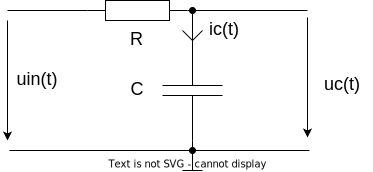
\includegraphics{SteuerRegel/images/Tiefpass.pdf}

}

\caption{\label{fig-Tiefpass}Tiefpass}

\end{figure}%

\begin{equation}\phantomsection\label{eq-ict_eq1}{
i_{c}{\left(t \right)} = \frac{\frac{d}{d t} u_{c}{\left(t \right)}}{C}
}\end{equation}

\begin{equation}\phantomsection\label{eq-ict_eq2}{
i_{c}{\left(t \right)} = \frac{- u_{c}{\left(t \right)} + u_{in}{\left(t \right)}}{R_{ohm}}
}\end{equation}

Durch Gleichsetzten von Gleichung~\ref{eq-ict_eq1} und
Gleichung~\ref{eq-ict_eq2} ergibt sich die allgemeine
Differenzialgleichung 1. Ordnung für den Tiefpass.

\begin{equation}\phantomsection\label{eq-RCTP}{
\frac{d}{d t} u_{c}{\left(t \right)} + \frac{u_{c}{\left(t \right)}}{C R_{ohm}} = \frac{u_{in}{\left(t \right)}}{C R_{ohm}}
}\end{equation}

\(R_{ohm}\) \ldots{} Ohmscher Widerstand

\(C\) \ldots{} Kapazität

\(t\) \ldots{} Zeit

\(u_{c}{\left(t \right)}\) \ldots{} Ausgangsspannung

\(i_{c}{\left(t \right)}\) \ldots{} Strom

\(u_{in}{\left(t \right)}\) \ldots{} Eingangsspannung

Müsste nun von dieser Differentialgleichung die Übertragungsfunktion,
also \(G=Ausgang/Eingang\), angegeben werden, so müsste zunächst die
Differentialgleichung gelöst werden.\\
Die Laplace Transformation bietet hier einen alternativen Weg der mit
weiteren Vorteilen verbunden ist wenn es darum geht Blöcke miteinander
zu kombinieren oder Aussagen über das System zu treffen.

\subsubsection{Laplacetransformation}\label{laplacetransformation}

Die tiefere Mathematik der Laplacetransofrmation überlassen wir hier den
Mathematiker:innen und den ersten Semstern eines Studiums. Wir wollen
die Laplacetransformation lediglich als Werkzeug zur vereinfachung
unserer Arbeit verwenden. Dazu benötigen wir folgende Grundregeln.\\
Vereinfacht ist die Laplacetransformation als eine Übersetzung aus dem
Zeitbereich, also mit der varaible \(t\), in den Frequenzbereich mit der
Variable \(s\) zu verstehen. Die Übersetzung erfolgt in vielen Fällen
sehr einfach mittels Tabelle. Hier wird die Transformation nur für
ausgewählte Signale und mathematische Operationen angeführt.

\begin{longtable}[]{@{}
  >{\raggedright\arraybackslash}p{(\columnwidth - 4\tabcolsep) * \real{0.1818}}
  >{\raggedright\arraybackslash}p{(\columnwidth - 4\tabcolsep) * \real{0.3182}}
  >{\raggedright\arraybackslash}p{(\columnwidth - 4\tabcolsep) * \real{0.5000}}@{}}
\caption{Laplacetransformationstabelle}\label{tbl-laplace}\tabularnewline
\toprule\noalign{}
\begin{minipage}[b]{\linewidth}\raggedright
Zeitbereich x(t)
\end{minipage} & \begin{minipage}[b]{\linewidth}\raggedright
Frequenzbereich X(s)
\end{minipage} & \begin{minipage}[b]{\linewidth}\raggedright
Bemerkung
\end{minipage} \\
\midrule\noalign{}
\endfirsthead
\toprule\noalign{}
\begin{minipage}[b]{\linewidth}\raggedright
Zeitbereich x(t)
\end{minipage} & \begin{minipage}[b]{\linewidth}\raggedright
Frequenzbereich X(s)
\end{minipage} & \begin{minipage}[b]{\linewidth}\raggedright
Bemerkung
\end{minipage} \\
\midrule\noalign{}
\endhead
\bottomrule\noalign{}
\endlastfoot
\(\frac{d \ x(t)}{d \ t}\) & \(s \cdot X(s) - x(0)\) & Transformation
der Ableitung nach der Zeit, \(x(0)\) ist dabei der Wert zum Zeitpunkt
Null. Bei einem Kondensator wäre dies zum Beispiel der Ladezustand zu
Beginn. \\
\({ \int x(t) \, d \ t}\) & \(\frac{1}{s} \cdot X(s)\) & Transformation
der Integration über der Zeit \\
\(\delta (t)\) & \(1\) & Transformation des Impulses \\
\(\sigma (t)\) & \(\frac{1}{s}\) & Transformation des Sprunges \\
\(e^{at}\) & \(\frac{1}{s -a}\) & \\
\(\frac{1}{a} e^{\frac{-t}{a}}\) & \(\frac{1}{1 + as}\) & \\
\end{longtable}

Wird nun Gleichung Gleichung~\ref{eq-RCTP} mittels der Tabelle
Tabelle~\ref{tbl-laplace} transformiert erhalten wir eine Gleichung aus
der wir durch einfaches Umformen eine Übertragungsfunktion erhalten. Es
wird angenommen, dass \$ x(0) = 0 \$ ist.

\begin{equation}\phantomsection\label{eq-Dummy}{
U_{C} s + \frac{U_{C}}{C R_{ohm}} = \frac{U_{IN}}{C R_{ohm}}
}\end{equation}

\begin{equation}\phantomsection\label{eq-Dummy}{
G = \frac{U_{C}}{U_{IN}}
}\end{equation}

\begin{equation}\phantomsection\label{eq-Dummy}{
G = \frac{1}{C R_{ohm} + s}
}\end{equation}

\subsection{Testsignale und Streckenverhalten}\label{sec-TestStrecke}

\subsubsection{Testsignale}\label{testsignale}

\subsubsection{Streckenverhalten}\label{streckenverhalten}

\paragraph{Interaktiver PT2 Simulator}\label{interaktiver-pt2-simulator}

\begin{Shaded}
\begin{Highlighting}[]
\NormalTok{//| echo: false}

\NormalTok{Plot.plot(\{}
\NormalTok{  y: \{}
\NormalTok{    grid: true,}
\NormalTok{  //  domain: [0, 4]}
\NormalTok{  \},}
\NormalTok{  marks: [}
\NormalTok{    Plot.line(y, \{}
\NormalTok{      x: "t",}
\NormalTok{      y: "s",}
\NormalTok{      stroke: \textquotesingle{}\#888\textquotesingle{}}
\NormalTok{    \}),}
\NormalTok{    Plot.line(y, \{ x: "t", y: "u", stroke: \textquotesingle{}\#34f\textquotesingle{} \})}
\NormalTok{  ]}
\NormalTok{\})}

\NormalTok{viewof input = Select(}
\NormalTok{  [\textquotesingle{}step\textquotesingle{}, \textquotesingle{}hardstep\textquotesingle{}, \textquotesingle{}smoothstep\textquotesingle{}, \textquotesingle{}ramp\textquotesingle{}, \textquotesingle{}quadratic ramp\textquotesingle{}],}
\NormalTok{  \{}
\NormalTok{    value: \textquotesingle{}step\textquotesingle{},}
\NormalTok{    label: \textquotesingle{}Input\textquotesingle{}}
\NormalTok{  \}}
\NormalTok{)}

\NormalTok{//viewof Kp = Range([1e{-}12, 100], \{}
\NormalTok{//  label: tex\textasciigrave{}K\_P\textasciigrave{},}
\NormalTok{//  value: 1,}
\NormalTok{//  transform: Math.log}
\NormalTok{//\})}

\NormalTok{//viewof Ki = Range([1e{-}12, 10], \{}
\NormalTok{//  label: tex\textasciigrave{}K\_I\textasciigrave{},}
\NormalTok{//  value: 0,}
\NormalTok{//  transform: Math.log}
\NormalTok{//\})}

\NormalTok{//viewof Kd = Range([1e{-}12, 1], \{}
\NormalTok{//  label: tex\textasciigrave{}K\_d\textasciigrave{},}
\NormalTok{//  value: 0,}
\NormalTok{//  transform: Math.log}
\NormalTok{//\})}

\NormalTok{//viewof dt = Range([1e{-}4, 0.1], \{}
\NormalTok{//  value: 0.001,}
\NormalTok{//  transform: Math.log,}
\NormalTok{//  label: tex\textasciigrave{}\textbackslash{}Delta t\textasciigrave{}}
\NormalTok{//\})}

\NormalTok{viewof Kpt2 = Range([1e{-}12, 5], \{}
\NormalTok{  value: 1,}
\NormalTok{  transform: Math.log,}
\NormalTok{  label: tex\textasciigrave{}K\_\{pt2\}\textasciigrave{}}
\NormalTok{\})}

\NormalTok{viewof D = Range([1e{-}12, 10], \{}
\NormalTok{  value: 0.5,}
\NormalTok{  transform: Math.log,}
\NormalTok{  label: tex\textasciigrave{}D\textasciigrave{}}
\NormalTok{\})}

\NormalTok{viewof T = Range([1e{-}12, 5], \{}
\NormalTok{  value: 1,}
\NormalTok{  transform: Math.log,}
\NormalTok{  label: tex\textasciigrave{}T\textasciigrave{}}
\NormalTok{\})}

\NormalTok{viewof tMax = Range([1, 10e3], \{}
\NormalTok{  value: 10,}
\NormalTok{  transform: Math.log,}
\NormalTok{  label: tex\textasciigrave{}t\_\{max\}\textasciigrave{}}
\NormalTok{\})}

\NormalTok{y = \{}
\NormalTok{  const output = [];}

\NormalTok{  let p; }
\NormalTok{  let t0 = {-}0.5;}
\NormalTok{  //let tMax = 20;}

\NormalTok{  let t = t0;}
\NormalTok{  let d = 0;}
\NormalTok{  let u = 0;}
\NormalTok{  let i = 0;}
\NormalTok{  let e = 0;}
\NormalTok{  let eprev = e;}
\NormalTok{  let pu = u;}
\NormalTok{  let ppu = u;}
\NormalTok{  let du = 0;}
\NormalTok{  let ddu = 0;}
\NormalTok{  let pdu = 0;}
\NormalTok{  let y = 0;}
\NormalTok{  let py = 0;}
\NormalTok{  let ppy = 0;}
\NormalTok{  let dy = 0;}
\NormalTok{  let ddy = 0;}
\NormalTok{  let pdy = 0;}
\NormalTok{  let de = 0;}
\NormalTok{  let dt = 0.001;}
\NormalTok{  let s = setPoint(t0);}
\NormalTok{  output.push(\{ t, u, s \});}

\NormalTok{  let j = 1;}
\NormalTok{  while (t \textless{} tMax) \{}
\NormalTok{    t = t0 + j * dt;}

\NormalTok{    s = setPoint(t);}
   
\NormalTok{    e = s {-} u;}
\NormalTok{    de = eprev{-}e;}

\NormalTok{    //du = (u{-}pu)/dt;}
\NormalTok{    //ddu = (du {-} pdu)/dt;}

\NormalTok{    //dy = (py {-} y)/dt;}
\NormalTok{    //ddy = (dy {-} pdy)/dt;}

\NormalTok{    p = e;}
\NormalTok{    i += e * dt;}
\NormalTok{    d = de/dt;}

\NormalTok{    y = s; //(Kp * p + Ki * i + Kd * d) * dt;}
    
\NormalTok{    u = (2*D*T*dt*pu + Kpt2*dt**2*y {-} T**2*ppu + 2*T**2*pu)/(2*D*T*dt + T**2 + dt**2);}

\NormalTok{    ppu = pu;}
\NormalTok{    pu = u;}
\NormalTok{    //pdu = du;}

\NormalTok{    //ppy = py;}
\NormalTok{    //py = y;}
\NormalTok{    //pdy = dy;}

\NormalTok{    eprev = e;}

\NormalTok{    output.push(\{ t, u, s \});}
\NormalTok{    j++;}
\NormalTok{  \}}

\NormalTok{  return output;}
\NormalTok{\}}

\NormalTok{setPoint = \{}
\NormalTok{  function hardstep(x) \{}
\NormalTok{    return Math.max(0, Math.min(1, x));}
\NormalTok{  \}}
\NormalTok{  function smoothstep(x) \{}
\NormalTok{    var x = hardstep(x);}
\NormalTok{    return x * x * (3 {-} 2 * x);}
\NormalTok{  \}}
\NormalTok{  switch (input) \{}
\NormalTok{    case \textquotesingle{}step\textquotesingle{}:}
\NormalTok{      return t =\textgreater{} (t \textgreater{}= 0 ? 1 : 0);}
\NormalTok{    case \textquotesingle{}ramp\textquotesingle{}:}
\NormalTok{      return t =\textgreater{} (t \textgreater{}= 0 ? t : 0);}
\NormalTok{    case \textquotesingle{}quadratic ramp\textquotesingle{}:}
\NormalTok{      return t =\textgreater{} (t \textgreater{}= 0 ? t * t : 0);}
\NormalTok{    case \textquotesingle{}smoothstep\textquotesingle{}:}
\NormalTok{      return smoothstep;}
\NormalTok{    case \textquotesingle{}hardstep\textquotesingle{}:}
\NormalTok{      return hardstep;}
\NormalTok{    default:}
\NormalTok{      throw new Error(\textquotesingle{}Invalid input\textquotesingle{});}
\NormalTok{  \}}
\NormalTok{\}}

\NormalTok{import \{ Range, Select \} from \textquotesingle{}@observablehq/inputs\textquotesingle{}}
\end{Highlighting}
\end{Shaded}

\subsubsection{Identifikation}\label{identifikation}

\subsection{Zusammenschaltung von
Blöcken}\label{zusammenschaltung-von-bluxf6cken}

Werden Blöcke kombiniert können die resultierenden
Übertragungsfunktionen berechnet werden.\\
Zur vereinfachung kann die Übertragungsfunktion des Sensors mit \(M=1\)
angenommen werden, \(M=1\), wenn dieser im Verhälnis zur Strecke und zum
Regler vernachlässigbar ist. Dies ist zum Beispiel der Fall wenn der
Sensor viel schneller ist als die Strecke und der Regler. Diese
Vorraussetzung ist für viele Systeme gegeben.

Für den Regelkreis, Abbildung~\ref{fig-Regelkreis}, ergebn sich folgende
Möglichkeiten.

\subsubsection{Die
Führungsübertragungsfunktion}\label{die-fuxfchrungsuxfcbertragungsfunktion}

Die Führungsübertragungsfunktion gibt das Verhältnis zwischen Sollgröße
und Istgröße an. Sie Beschreibt damit das Verhalten des Regelkreises mit
der Sollgröße als Eingang und der Istgröße als Ausgang. Ist eine
Regelstrecke ideal so ist die die Führungsübertragungsfunktion gleich
Eins.

\begin{equation}\phantomsection\label{eq-Fw_eq}{
F_{w} = \frac{G R}{G M R + 1}
}\end{equation}

\(F_{w}\) \ldots{} Führungsübertragungsfunktion

\subsubsection{Die
Schleifenübertragungsfunktion}\label{die-schleifenuxfcbertragungsfunktion}

Die Schleifenübertragungsfunktion ist die Übertragungsfunktion des
offenen Regelkreises, also ohne Rückkopplung und ist im Laplace Bereich
eine einfache Multiplikation.

\begin{equation}\phantomsection\label{eq-Dummy}{
F_{o} = G R
}\end{equation}

\(F_{o}\) \ldots{} Schleifenübertragungsfunktion

\subsubsection{Die
Störübertragungsfunktion}\label{die-stuxf6ruxfcbertragungsfunktion}

Die Störübertragungsfunktion beschreibt wie sich die Störgröße auf den
Ausgang auswirkt.

\begin{equation}\phantomsection\label{eq-Dummy}{
F_{s} = \frac{G}{F_{o} + 1}
}\end{equation}

\(F_{s}\) \ldots{} Störübertragungsfunktion

\subsection{Interaktiver PID
Simulator}\label{interaktiver-pid-simulator}

{ Eingangssignal \(w\) }\\
{ Ausgangssignal \(y\) }\\
{ Regelabweichung \(e\) }\\
{ Stellgröße \(u\) }

\begin{Shaded}
\begin{Highlighting}[]
\NormalTok{// The basic code layout was found on source: https://observablehq.com/@mbostock/inputs}
\NormalTok{// be aware, the code variables do not yet match the variable names in the document}

\NormalTok{Plot.plot(\{}
\NormalTok{  y: \{}
\NormalTok{    grid: true,}
\NormalTok{  //  domain: [0, 4]}
\NormalTok{  \},}
\NormalTok{  marks: [}
\NormalTok{    Plot.line(y\_PID, \{}
\NormalTok{      x: "t\_PID",}
\NormalTok{      y: "s\_PID",}
\NormalTok{      stroke: \textquotesingle{}\#888\textquotesingle{}}
\NormalTok{    \}),}
\NormalTok{    Plot.line(y\_PID, \{ x: "t\_PID", y: "u\_PID", stroke: \textquotesingle{}\#34f\textquotesingle{} \}), //BLue}
\NormalTok{    Plot.line(y\_PID, \{ x: "t\_PID", y: "e\_PID", stroke: \textquotesingle{}\#fb2f03\textquotesingle{} \}), //RED}
\NormalTok{    Plot.line(y\_PID, \{ x: "t\_PID", y: "y\_PID", stroke: \textquotesingle{}\#d7fb03\textquotesingle{} \}),  //Greenisch}
\NormalTok{  ]}
\NormalTok{\})}
\end{Highlighting}
\end{Shaded}

Reglereinstellungen:

\begin{Shaded}
\begin{Highlighting}[]

\NormalTok{viewof Kp\_PID = Range([1e{-}12, 10e3], \{}
\NormalTok{  label: tex\textasciigrave{}K\_P\textasciigrave{},}
\NormalTok{  value: 1,}
\NormalTok{  transform: Math.log}
\NormalTok{\})}

\NormalTok{viewof Ki\_PID = Range([1e{-}12, 10e2], \{}
\NormalTok{  label: tex\textasciigrave{}K\_I\textasciigrave{},}
\NormalTok{  value: 0,}
\NormalTok{  transform: Math.log}
\NormalTok{\})}

\NormalTok{viewof Kd\_PID = Range([1e{-}12, 10e1], \{}
\NormalTok{  label: tex\textasciigrave{}K\_d\textasciigrave{},}
\NormalTok{  value: 0,}
\NormalTok{  transform: Math.log}
\NormalTok{\})}

\NormalTok{//viewof dt = Range([1e{-}4, 0.1], \{}
\NormalTok{//  value: 0.001,}
\NormalTok{//  transform: Math.log,}
\NormalTok{//  label: tex\textasciigrave{}\textbackslash{}Delta t\textasciigrave{}}
\NormalTok{//\})}
\end{Highlighting}
\end{Shaded}

Streckeneinstellungen:

\begin{Shaded}
\begin{Highlighting}[]

\NormalTok{viewof Kpt2\_PID = Range([1e{-}12, 10e3], \{}
\NormalTok{  value: 1,}
\NormalTok{  transform: Math.log,}
\NormalTok{  label: tex\textasciigrave{}K\_\{pt2\}\textasciigrave{}}
\NormalTok{\})}

\NormalTok{viewof D\_PID = Range([1e{-}12, 10], \{}
\NormalTok{  value: 1,}
\NormalTok{  transform: Math.log,}
\NormalTok{  label: tex\textasciigrave{}D\textasciigrave{}}
\NormalTok{\})}

\NormalTok{viewof T\_PID = Range([1e{-}12, 5], \{}
\NormalTok{  value: 1,}
\NormalTok{  transform: Math.log,}
\NormalTok{  label: tex\textasciigrave{}T\textasciigrave{}}
\NormalTok{\})}
\end{Highlighting}
\end{Shaded}

Auswahl Eingangssignal:

\begin{Shaded}
\begin{Highlighting}[]

\NormalTok{viewof input\_PID = Select(}
\NormalTok{  [\textquotesingle{}step\textquotesingle{}, \textquotesingle{}hardstep\textquotesingle{}, \textquotesingle{}smoothstep\textquotesingle{}, \textquotesingle{}ramp\textquotesingle{}, \textquotesingle{}quadratic ramp\textquotesingle{}],}
\NormalTok{  \{}
\NormalTok{    value: \textquotesingle{}step\textquotesingle{},}
\NormalTok{    label: \textquotesingle{}Input\textquotesingle{}}
\NormalTok{  \}}
\NormalTok{)}
\end{Highlighting}
\end{Shaded}

Simulationseinstellungen:

\begin{Shaded}
\begin{Highlighting}[]

\NormalTok{viewof tMax\_PID = Range([1, 10e3], \{}
\NormalTok{  value: 10,}
\NormalTok{  transform: Math.log,}
\NormalTok{  label: tex\textasciigrave{}t\_\{max\}\textasciigrave{}}
\NormalTok{\})}

\NormalTok{y\_PID = \{}
\NormalTok{  const output\_PID = [];}

\NormalTok{  let p\_PID; }
\NormalTok{  let t0\_PID = {-}0.5;}
\NormalTok{  //let tMax\_PID = 20;}

\NormalTok{  let t\_PID = t0\_PID;}
\NormalTok{  let d\_PID = 0;}
\NormalTok{  let u\_PID = 0;}
\NormalTok{  let i\_PID = 0;}
\NormalTok{  let e\_PID = 0;}
\NormalTok{  let eprev\_PID = e\_PID;}
\NormalTok{  let pu\_PID = u\_PID;}
\NormalTok{  let ppu\_PID = u\_PID;}
\NormalTok{  let du\_PID = 0;}
\NormalTok{  let ddu\_PID = 0;}
\NormalTok{  let pdu\_PID = 0;}
\NormalTok{  let y\_PID = 0;}
\NormalTok{  let py\_PID = 0;}
\NormalTok{  let ppy\_PID = 0;}
\NormalTok{  let dy\_PID = 0;}
\NormalTok{  let ddy\_PID = 0;}
\NormalTok{  let pdy\_PID = 0;}
\NormalTok{  let de\_PID = 0;}
\NormalTok{  let dt\_PID = 0.001;}
\NormalTok{  let s\_PID = setPoint(t0\_PID);}
\NormalTok{  output\_PID.push(\{ t\_PID, u\_PID, s\_PID \});}

\NormalTok{  let j\_PID = 1;}
\NormalTok{  while (t\_PID \textless{} tMax\_PID) \{}
\NormalTok{    t\_PID = t0\_PID + j\_PID * dt\_PID;}

\NormalTok{    s\_PID = setPoint\_PID(t\_PID);}
   
\NormalTok{    e\_PID = s\_PID {-} u\_PID;}
\NormalTok{    de\_PID = eprev\_PID{-}e\_PID;}

\NormalTok{    //du = (u{-}pu)/dt;}
\NormalTok{    //ddu = (du {-} pdu)/dt;}

\NormalTok{    //dy = (py {-} y)/dt;}
\NormalTok{    //ddy = (dy {-} pdy)/dt;}

\NormalTok{    p\_PID = e\_PID;}
\NormalTok{    i\_PID += e\_PID * dt\_PID;}
\NormalTok{    d\_PID = de\_PID/dt\_PID;}

\NormalTok{    y\_PID = (Kp\_PID * p\_PID + Ki\_PID * i\_PID + Kd\_PID * d\_PID);}
    
\NormalTok{    u\_PID = (2*D\_PID*T\_PID*dt\_PID*pu\_PID + Kpt2\_PID*dt\_PID**2*y\_PID {-} T\_PID**2*ppu\_PID + 2*T\_PID**2*pu\_PID)/(2*D\_PID*T\_PID*dt\_PID + T\_PID**2 + dt\_PID**2);}

\NormalTok{    ppu\_PID = pu\_PID;}
\NormalTok{    pu\_PID = u\_PID;}
\NormalTok{    //pdu = du;}

\NormalTok{    //ppy = py;}
\NormalTok{    //py = y;}
\NormalTok{    //pdy = dy;}

\NormalTok{    eprev\_PID = e\_PID;}

\NormalTok{    output\_PID.push(\{ t\_PID, u\_PID, s\_PID, e\_PID, y\_PID \});}
\NormalTok{    j\_PID++;}
\NormalTok{  \}}

\NormalTok{  return output\_PID;}
\NormalTok{\}}

\NormalTok{setPoint\_PID = \{}
\NormalTok{  function hardstep\_PID(x) \{}
\NormalTok{    return Math.max(0, Math.min(1, x));}
\NormalTok{  \}}
\NormalTok{  function smoothstep\_PID(x) \{}
\NormalTok{    var x = hardstep\_PID(x);}
\NormalTok{    return x * x * (3 {-} 2 * x);}
\NormalTok{  \}}
\NormalTok{  switch (input) \{}
\NormalTok{    case \textquotesingle{}step\textquotesingle{}:}
\NormalTok{      return t\_PID =\textgreater{} (t\_PID \textgreater{}= 0 ? 1 : 0);}
\NormalTok{    case \textquotesingle{}ramp\textquotesingle{}:}
\NormalTok{      return t\_PID =\textgreater{} (t\_PID \textgreater{}= 0 ? t\_PID : 0);}
\NormalTok{    case \textquotesingle{}quadratic ramp\textquotesingle{}:}
\NormalTok{      return t\_PID =\textgreater{} (t\_PID \textgreater{}= 0 ? t\_PID * t\_PID : 0);}
\NormalTok{    case \textquotesingle{}smoothstep\textquotesingle{}:}
\NormalTok{      return smoothstep\_PID;}
\NormalTok{    case \textquotesingle{}hardstep\textquotesingle{}:}
\NormalTok{      return hardstep\_PID;}
\NormalTok{    default:}
\NormalTok{      throw new Error(\textquotesingle{}Invalid input\textquotesingle{});}
\NormalTok{  \}}
\NormalTok{\}}

\NormalTok{//import \{ Range, Select \} from \textquotesingle{}@observablehq/inputs\textquotesingle{}}
\end{Highlighting}
\end{Shaded}

\bookmarksetup{startatroot}

\chapter*{References}\label{references}
\addcontentsline{toc}{chapter}{References}

\markboth{References}{References}

\phantomsection\label{refs}
\begin{CSLReferences}{0}{1}
\end{CSLReferences}



\end{document}
